% Native publication figure. Requires tikz; use the coordinate list as its text equivalent.
\begin{figure}[htbp]
  \centering
  \begingroup
  \newcommand{\LifeGrid}[2]{%
    \begin{scope}[xshift=#1]
      \foreach \x/\y in {#2} \fill (\x-0.5,\y-0.5) rectangle (\x+0.5,\y+0.5);
      \foreach \k in {0,...,8} {
          \draw[gray] (\k-0.5,-0.5)--(\k-0.5,7.5);
          \draw[gray] (-0.5,\k-0.5)--(7.5,\k-0.5);
        }
    \end{scope}}
  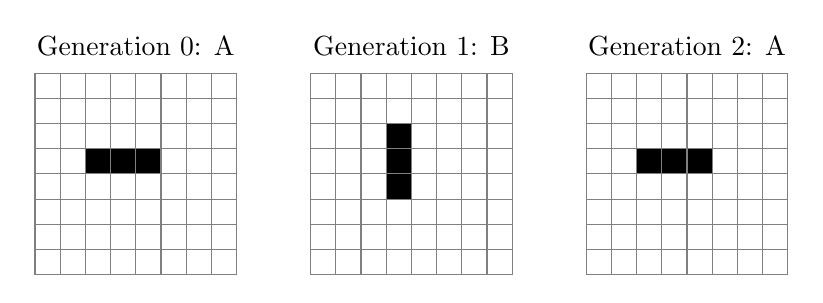
\begin{tikzpicture}[x=0.32cm,y=-0.32cm]
    \LifeGrid{0cm}{2/3,3/3,4/3}
    \LifeGrid{3.5cm}{3/2,3/3,3/4}
    \LifeGrid{7cm}{2/3,3/3,4/3}
    \node[above] at (3.5,-0.8) {Generation 0: A};
    \node[above] at (14.4375,-0.8) {Generation 1: B};
    \node[above] at (25.375,-0.8) {Generation 2: A};
  \end{tikzpicture}
  \endgroup
  \caption{A three-cell oscillator through two synchronous updates. Filled cells are alive. The current allocation alternates A, B, A even though generation two repeats the initial image.}
  \label{fig:life-oscillator}
\end{figure}
